% ====================================================================================
\chapter{对偶理论：换个角度看问题}
% ====================================================================================

\section*{一个迟到的研究生}

\marginnote{\textbf{乔治·丹齐格}(1914--2005)：线性规划之父，单纯形法发明人。他``误把未解决问题当作业解决''的故事成为传奇，启发了电影《心灵捕手》。1975年获美国国家科学奖章，被誉为``20世纪最重要的应用数学家之一''。}

1939年秋天的一个清晨，加州大学伯克利分校的研究生George Dantzig迟到了。当他匆忙走进统计学课堂时，Jerzy Neyman教授正在黑板上写着两道题目。Dantzig以为那是这周的作业，就把题目抄下来了。

接下来的几天，Dantzig发现这两道"作业"异常困难。但他没有放弃，花了好几个晚上反复尝试。几天后，他把解答交给教授，有些尴尬地说："这作业有点难，我花了不少时间。能不能宽限一下？"

Neyman教授看着解答，沉默了很久。然后他说出了一句让Dantzig震惊的话：

"这不是作业。这是我在课上提到的两个\textbf{著名的未解决问题}，用来说明统计学前沿有多困难。你……把它们都解决了。"

\clarify{这个故事后来成为电影《心灵捕手》的灵感来源。Dantzig因为不知道问题是"不可能的"，所以没有心理障碍，反而解决了它们。}

\section*{从战争中诞生的对偶理论}

1947年，第二次世界大战刚刚结束。美国空军面临一个巨大的后勤难题：如何以最低成本调度数千架飞机、协调数百个基地的物资供应？

Dantzig被指派解决这个问题。他首先将问题形式化为\textbf{线性规划}（Linear Programming），然后发现了一个惊人的事实：

\begin{center}
\fbox{\parbox{0.9\textwidth}{
每一个优化问题都有一个"镜像"版本。原问题问的是"用多少资源"，镜像问题问的是"资源值多少钱"。

神奇的是：这两个问题的最优值\textbf{相等}！更妙的是：有时候镜像问题比原问题\textbf{更容易求解}。
}}
\end{center}

这就是\textbf{对偶理论}的起源。它不是纯数学的抽象游戏，而是从实际的军事后勤问题中诞生的。

\vspace{0.5cm}
\noindent\textit{想象你是一个快递公司的调度员，需要优化100辆货车的路线。直接求解需要考虑$100!$种可能——这个数字比宇宙中的原子数还多。但如果换个角度，从"每条路的使用成本"来思考，问题可能突然变得简单了。}

\begin{quote}
\textbf{本章目标}：理解为什么有时候"绕个弯"反而更快——对偶问题可能比原问题更容易求解。这不仅是计算技巧，更是拉格朗日乘子法的自然延伸。
\end{quote}

\begin{tcolorbox}[colback=green!5, colframe=green!60!black, title=学完这章，你将能够...]
\begin{itemize}
    \item 写出任意优化问题的对偶问题
    \item 利用弱对偶性获得原问题的下界（用于算法验证）
    \item 判断何时强对偶成立，从而用对偶问题替代原问题求解
    \item 理解SVM、最大熵模型等机器学习算法背后的对偶结构
    \item 用互补松弛条件从对偶解恢复原问题的解
\end{itemize}
\end{tcolorbox}

% ------------------------------------------------------------------------------------
\section{从拉格朗日函数到对偶}

\subsection{回顾：拉格朗日函数}

在第1章，我们学习了拉格朗日函数：
\[
\Lag(x, \lambda) = f(x) + \lambda^\top g(x)
\]

关键洞察是：对于满足约束$g(x) = 0$的点，$\Lag$和$f$的取值完全一样。

现在我们要问一个新问题：这个函数有两个变量$x$和$\lambda$，如果要找它的"最优点"，应该怎么办？

\subsection{两种优化顺序}

拉格朗日函数$\Lag(x, \lambda)$是两组变量的函数。一个自然的问题是：我们应该先优化$x$还是先优化$\lambda$？

答案是：\textbf{先优化谁，结果可能不一样！}

\textbf{顺序A}：先固定$\lambda$，对$x$求最小值；然后再对$\lambda$求最大值
\[
\max_\lambda \min_x \Lag(x, \lambda)
\]

\textbf{顺序B}：先固定$x$，对$\lambda$求最大值；然后再对$x$求最小值
\[
\min_x \max_\lambda \Lag(x, \lambda)
\]

\textbf{关键问题}：这两种顺序得到的结果一样吗？

让我们通过两个例子来看。

\subsubsection{例1：矩阵博弈}

考虑一个资源分配问题。行玩家（攻方）选择进攻方向$i \in \{1,2,3,4\}$，列玩家（守方）选择防守位置$j \in \{1,2,3,4\}$。矩阵元素$a_{ij}$表示攻方的损失：

\[
A = \begin{pmatrix}
7 & 2 & 5 & 9 \\
3 & 6 & 8 & 4 \\
5 & 4 & 3 & 7 \\
6 & 8 & 4 & 2
\end{pmatrix}
\]

攻方想让损失\textbf{最小}，守方想让攻方损失\textbf{最大}。

\vspace{0.3cm}
\textbf{顺序A}：$\max_j \min_i a_{ij}$（守方先选，攻方后选）

\begin{center}
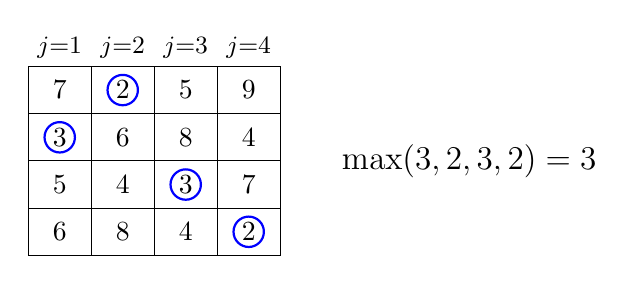
\begin{tikzpicture}[scale=0.8]
    % 矩阵框架
    \draw (0, 0) rectangle (4, 3);
    \draw (1, 0) -- (1, 3); \draw (2, 0) -- (2, 3); \draw (3, 0) -- (3, 3);
    \draw (0, 0.75) -- (4, 0.75); \draw (0, 1.5) -- (4, 1.5); \draw (0, 2.25) -- (4, 2.25);
    
    % 列标签
    \node[font=\small] at (0.5, 3.3) {$j$=1}; \node[font=\small] at (1.5, 3.3) {$j$=2}; 
    \node[font=\small] at (2.5, 3.3) {$j$=3}; \node[font=\small] at (3.5, 3.3) {$j$=4};
    
    % 矩阵元素，高亮每列最小值
    \node at (0.5, 2.625) {7}; \node at (1.5, 2.625) {\tikz\node[circle,draw=blue,thick,inner sep=1pt]{2};}; \node at (2.5, 2.625) {5}; \node at (3.5, 2.625) {9};
    \node at (0.5, 1.875) {\tikz\node[circle,draw=blue,thick,inner sep=1pt]{3};}; \node at (1.5, 1.875) {6}; \node at (2.5, 1.875) {8}; \node at (3.5, 1.875) {4};
    \node at (0.5, 1.125) {5}; \node at (1.5, 1.125) {4}; \node at (2.5, 1.125) {\tikz\node[circle,draw=blue,thick,inner sep=1pt]{3};}; \node at (3.5, 1.125) {7};
    \node at (0.5, 0.375) {6}; \node at (1.5, 0.375) {8}; \node at (2.5, 0.375) {4}; \node at (3.5, 0.375) {\tikz\node[circle,draw=blue,thick,inner sep=1pt]{2};};
    

    % 箭头和最终结果
    \node[font=\large\bfseries] at (7, 1.5) {$\max(3,2,3,2) = \boxed{3}$};
\end{tikzpicture}
\end{center}

\textbf{顺序B}：$\min_i \max_j a_{ij}$（攻方先选，守方后选）

\begin{center}
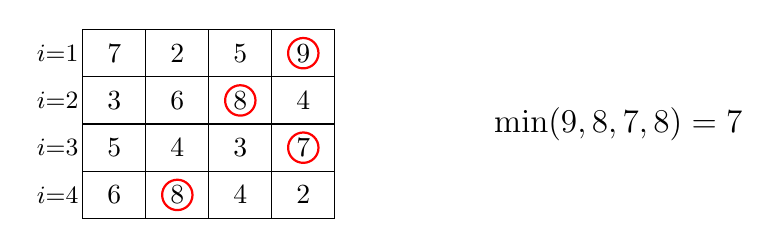
\begin{tikzpicture}[scale=0.8]
    % 矩阵框架
    \draw (0, 0) rectangle (4, 3);
    \draw (1, 0) -- (1, 3); \draw (2, 0) -- (2, 3); \draw (3, 0) -- (3, 3);
    \draw (0, 0.75) -- (4, 0.75); \draw (0, 1.5) -- (4, 1.5); \draw (0, 2.25) -- (4, 2.25);
    
    % 行标签
    \node[font=\small] at (-0.4, 2.625) {$i$=1}; \node[font=\small] at (-0.4, 1.875) {$i$=2}; 
    \node[font=\small] at (-0.4, 1.125) {$i$=3}; \node[font=\small] at (-0.4, 0.375) {$i$=4};
    
    % 矩阵元素，高亮每行最大值
    \node at (0.5, 2.625) {7}; \node at (1.5, 2.625) {2}; \node at (2.5, 2.625) {5}; \node at (3.5, 2.625) {\tikz\node[circle,draw=red,thick,inner sep=1pt]{9};};
    \node at (0.5, 1.875) {3}; \node at (1.5, 1.875) {6}; \node at (2.5, 1.875) {\tikz\node[circle,draw=red,thick,inner sep=1pt]{8};}; \node at (3.5, 1.875) {4};
    \node at (0.5, 1.125) {5}; \node at (1.5, 1.125) {4}; \node at (2.5, 1.125) {3}; \node at (3.5, 1.125) {\tikz\node[circle,draw=red,thick,inner sep=1pt]{7};};
    \node at (0.5, 0.375) {6}; \node at (1.5, 0.375) {\tikz\node[circle,draw=red,thick,inner sep=1pt]{8};}; \node at (2.5, 0.375) {4}; \node at (3.5, 0.375) {2};
    

    % 箭头和最终结果
    \node[font=\large\bfseries] at (8.5, 1.5) {$\min(9,8,7,8) = \boxed{7}$};
\end{tikzpicture}
\end{center}

\vspace{0.2cm}
\begin{center}
\fbox{\parbox{0.85\textwidth}{
\textbf{结论}：$\displaystyle\max_j \min_i = 3 \neq 7 = \min_i \max_j$

两种顺序差了4！后行动的玩家能看到对方的选择再做决策，天然占优势。
}}
\end{center}


\subsubsection{例2：连续函数}

考虑函数
\[
F(x, y) = -x^2 + xy, \quad x \in \R, \; y \in [-2, 2]
\]

\textbf{顺序A}：$\displaystyle\max_{y \in [-2,2]} \min_{x \in \R} (-x^2 + xy)$

\begin{center}
\begin{tikzpicture}[scale=0.8]
    % Step 1: 固定y，对x求min
    \node[blue, font=\bfseries] at (0, 3) {Step 1: 固定$y$，对$x$求$\min$};
    
    \node at (0, 2.2) {$\displaystyle\pd{F}{x} = -2x + y = 0 \;\Rightarrow\; x^* = \frac{y}{2}$};
    
    \node at (0, 1.2) {代入：$\displaystyle F\Big(\frac{y}{2}, y\Big) = -\frac{y^2}{4} + \frac{y^2}{2} = \frac{y^2}{4}$};
    
    % Step 2
    \node[red, font=\bfseries] at (0, 0) {Step 2: 对$y$求$\max$};
    
    \node at (0, -0.9) {$\displaystyle\max_{y \in [-2,2]} \frac{y^2}{4} = \frac{4}{4} = 1$（在$y = \pm 2$）};
    
    \draw[thick, ->] (4, 1) -- (5.5, 1);
    \node[font=\Large\bfseries, red] at (7, 1) {结果 $= 1$};
\end{tikzpicture}
\end{center}

\textbf{顺序B}：$\displaystyle\min_{x \in \R} \max_{y \in [-2,2]} (-x^2 + xy)$

\begin{center}
\begin{tikzpicture}[scale=0.8]
    % Step 1: 固定x，对y求max
    \node[blue, font=\bfseries] at (0, 3) {Step 1: 固定$x$，对$y$求$\max$};
    
    \node at (0, 2.1) {$F = -x^2 + xy$ 关于$y$是线性的};
    
    \node at (0, 0.5) {$\begin{cases} x > 0: & \max\text{在 } y=2, \; F = -x^2 + 2x \\ x < 0: & \max\text{在 } y=-2, \; F = -x^2 - 2x \\ x = 0: & F = 0 \end{cases}$};
    
    % Step 2
    \node[red, font=\bfseries] at (0, -1.3) {Step 2: 对$x$求$\min$};
    
    \node at (0, -2.2) {$\displaystyle\max_y F = -x^2 + 2|x| = -(|x|-1)^2 + 1$};
    
    \node at (0, -3.5) {这是开口向下的抛物线，最大值$1$在$|x|=1$，最小值$0$在$x=0$};
    
    \draw[thick, ->] (4.5, -4) -- (6, -4);
    \node[font=\Large\bfseries, red] at (7.5, -4) {结果 $= 0$};
\end{tikzpicture}
\end{center}

% 画函数图
\begin{figure}[h]
\centering
\begin{tikzpicture}[scale=0.9]
    % 左图：顺序A
    \begin{scope}[xshift=0cm]
        \draw[->] (-2.5, 0) -- (2.5, 0) node[right] {$y$};
        \draw[->] (0, -0.5) -- (0, 1.5) node[above] {$g(y)$};
        \draw[thick, blue, domain=-2:2, samples=50] plot (\x, {\x*\x/4});
        \fill[red] (-2, 1) circle (2pt);
        \fill[red] (2, 1) circle (2pt);
        \node[below] at (0, -0.8) {$g(y) = y^2/4$};
        \node[red, right] at (2.1, 1) {\small $\max = 1$};
        \node[below] at (0, -1.5) {\textbf{顺序A}：$\max_y g(y) = 1$};
    \end{scope}
    
    % 右图：顺序B
    \begin{scope}[xshift=7cm]
        \draw[->] (-2.5, 0) -- (2.5, 0) node[right] {$x$};
        \draw[->] (0, -0.5) -- (0, 1.5) node[above] {$h(x)$};
        \draw[thick, blue, domain=-2:0, samples=50] plot (\x, {-\x*\x - 2*\x});
        \draw[thick, blue, domain=0:2, samples=50] plot (\x, {-\x*\x + 2*\x});
        \fill[red] (0, 0) circle (2pt);
        \fill[blue] (-1, 1) circle (2pt);
        \fill[blue] (1, 1) circle (2pt);
        \node[below] at (0, -0.8) {$h(x) = -x^2 + 2|x|$};
        \node[red, right] at (0.1, -0.2) {\small $\min = 0$};
        \node[below] at (0, -1.5) {\textbf{顺序B}：$\min_x h(x) = 0$};
    \end{scope}
\end{tikzpicture}
\caption{两种优化顺序得到不同的中间函数，最终结果也不同}
\end{figure}

\begin{center}
\fbox{\parbox{0.85\textwidth}{
\textbf{结论}：$\displaystyle\max_y \min_x F = 1 \neq 0 = \min_x \max_y F$

同样的函数，不同的优化顺序，差了1！
}}
\end{center}

\subsubsection{规律总结}

\begin{center}
\begin{tikzpicture}
    \draw[thick, rounded corners, fill=blue!10] (0, 0) rectangle (6.5, 2.5);
    \node[font=\bfseries] at (3.25, 2) {Max-Min 不等式};
    \node at (3.25, 1.2) {$\displaystyle\max_y \min_x F(x,y) \;\leq\; \min_x \max_y F(x,y)$};
    \node[font=\small] at (3.25, 0.4) {后行动者占优势，结果更有利于他};
\end{tikzpicture}
\end{center}

\textbf{直观理解}：后行动的玩家能\textbf{看到对方的选择再决策}，所以总是占优势。

\begin{itemize}
    \item 顺序A中，$y$先选，$x$后选——$x$占优势，能把结果压低
    \item 顺序B中，$x$先选，$y$后选——$y$占优势，能把结果抬高
    \item 所以顺序A的结果 $\leq$ 顺序B的结果
\end{itemize}

\begin{insightbox}
\textbf{对偶间隙}：把这个不等式应用到拉格朗日函数：
\[
\underbrace{\max_\lambda \min_x \Lag(x, \lambda)}_{\text{对偶问题最优值}} \;\leq\; \underbrace{\min_x \max_\lambda \Lag(x, \lambda)}_{\text{原问题最优值}}
\]
左右两边的差叫做\textbf{对偶间隙}（duality gap）。

对于\textbf{凸优化}问题，在适当条件下（Slater条件），对偶间隙为零——这就是\textbf{强对偶性}，意味着两种顺序给出相同结果。
\end{insightbox}



\section{博弈论视角：对偶的直觉来源}

\subsection{一个思想实验}

在深入数学推导之前，让我们先用一个博弈的比喻来理解对偶的本质。

想象 $x$ 和 $\lambda$ 是两个玩家在玩一个\textbf{零和博弈}。他们面对同一个函数——拉格朗日函数 $\mathcal{L}(x, \lambda)$，但目标相反：

\begin{itemize}
    \item \textbf{玩家 $x$}：想让 $\mathcal{L}$ 尽量\textbf{小}（他是"最小化者"）
    \item \textbf{玩家 $\lambda$}：想让 $\mathcal{L}$ 尽量\textbf{大}（他是"最大化者"）
\end{itemize}

现在问一个关键问题：\textbf{谁先出牌？}

\subsection{先手劣势}

在大多数博弈中，先出牌的人会吃亏——因为后手可以看到先手的选择，然后针对性地做出最优响应。

\begin{example}[石头剪刀布]
如果你先出，对方后出，你永远赢不了。对方看到你出石头，就出布；看到你出剪刀，就出石头。

先手必败，后手必胜。
\end{example}

\begin{example}[讨价还价]
买卖双方谈判。如果卖家先报价，买家可以针对这个价格压价；如果买家先出价，卖家可以针对性地抬高。

谁先开口，谁就暴露了自己的底线。
\end{example}

同样的道理适用于 $x$ 和 $\lambda$ 的博弈：

\begin{center}
\renewcommand{\arraystretch}{1.5}
\begin{tabular}{c|c|c}
\toprule
 & \textbf{$x$ 先出牌} & \textbf{$\lambda$ 先出牌} \\
\midrule
数学表达 & $\displaystyle\min_x \max_\lambda \mathcal{L}(x,\lambda)$ & $\displaystyle\max_\lambda \min_x \mathcal{L}(x,\lambda)$ \\
\midrule
谁吃亏？ & $x$ 吃亏 & $\lambda$ 吃亏 \\
\midrule
为什么？ & $\lambda$ 看到 $x$ 的选择后， & $x$ 看到 $\lambda$ 的选择后， \\
 & 可以选最大的 $\mathcal{L}$ & 可以选最小的 $\mathcal{L}$ \\
\bottomrule
\end{tabular}
\end{center}

\subsection{弱对偶定理的直觉}

既然先手吃亏，那么：

\begin{itemize}
    \item 当 $x$ 先出牌时，$\lambda$ 可以把 $\mathcal{L}$ 推高 $\Rightarrow$ 结果偏大
    \item 当 $\lambda$ 先出牌时，$x$ 可以把 $\mathcal{L}$ 压低 $\Rightarrow$ 结果偏小
\end{itemize}

所以必然有：
\[
\underbrace{\min_x \max_\lambda \mathcal{L}(x,\lambda)}_{x\text{ 先出牌，吃亏，结果大}} \;\geq\; \underbrace{\max_\lambda \min_x \mathcal{L}(x,\lambda)}_{\lambda\text{ 先出牌，吃亏，结果小}}
\]

这就是\textbf{弱对偶定理}！

\begin{keytheorem}[title=弱对偶定理]
对于任何函数 $\mathcal{L}(x, \lambda)$：
\[
\min_x \max_\lambda \mathcal{L} \;\geq\; \max_\lambda \min_x \mathcal{L}
\]

左边称为\textbf{原始问题}的最优值，右边称为\textbf{对偶问题}的最优值。

弱对偶说：原始最优值 $\geq$ 对偶最优值。
\end{keytheorem}

\subsection{强对偶：什么时候先后手无所谓？}

弱对偶告诉我们 $\min\max \geq \max\min$。但在某些"好的"问题中，两者相等！

\begin{keytheorem}[title=强对偶定理（非正式版）]
如果原始问题是\textbf{凸优化问题}，并且满足一定的正则条件（如 Slater 条件），则：
\[
\min_x \max_\lambda \mathcal{L} \;=\; \max_\lambda \min_x \mathcal{L}
\]

这意味着：无论谁先出牌，最终的博弈结果是一样的！
\end{keytheorem}

\begin{physicalmeaning}
强对偶成立时，博弈达到了\textbf{纳什均衡}——双方都没有动机单方面改变策略。

在经济学中，这对应于\textbf{市场均衡}：买家的出价恰好等于卖家能接受的最低价，双方都无法通过单方面改变获得更好的结果。
\end{physicalmeaning}

\begin{insightbox}
\textbf{弱对偶}：$\min\max \geq \max\min$，先手吃亏。这对任何问题都成立。

\textbf{强对偶}：$\min\max = \max\min$，先后手无所谓。这对"好的"凸问题成立。

强对偶是优化理论中最深刻的结果之一——它让我们可以选择更容易求解的那个问题（原始或对偶）。
\end{insightbox}

% ------------------------------------------------------------------------------------
\section{从拉格朗日函数推导对偶问题}

博弈论的直觉告诉我们对偶的"why"。现在让我们看看具体的"how"——对偶问题是怎么从拉格朗日函数一步步推导出来的。

\subsection{一个具体的线性规划问题}

考虑一个工厂的生产决策问题：

\begin{example}[家具厂的困境]
一家家具厂生产桌子和椅子。

\textbf{已知信息}：
\begin{itemize}
    \item 每张桌子利润 300 元，需要 4 小时木工、2 小时油漆
    \item 每把椅子利润 200 元，需要 2 小时木工、3 小时油漆
    \item 本周可用：木工 100 小时，油漆 90 小时
\end{itemize}

\textbf{决策}：生产多少桌子（$x_1$）和椅子（$x_2$）？
\end{example}

这是一个标准的线性规划：
\[
\max_{x_1, x_2} \quad 300 x_1 + 200 x_2
\]
\[
\text{s.t.} \quad 4x_1 + 2x_2 \leq 100 \quad \text{（木工时间）}
\]
\[
2x_1 + 3x_2 \leq 90 \quad \text{（油漆时间）}
\]
\[
x_1, x_2 \geq 0
\]

用矩阵形式写成：
\[
\max_x \; c^\top x \quad \text{s.t.} \quad Ax \leq b, \; x \geq 0
\]

其中：
\[
c = \begin{pmatrix} 300 \\ 200 \end{pmatrix}, \quad
A = \begin{pmatrix} 4 & 2 \\ 2 & 3 \end{pmatrix}, \quad
b = \begin{pmatrix} 100 \\ 90 \end{pmatrix}
\]

\subsection{构造拉格朗日函数}

对约束 $Ax \leq b$ 引入拉格朗日乘子 $y \geq 0$（不等式约束的乘子必须非负，第1章讲过）：

\[
\mathcal{L}(x, y) = c^\top x + y^\top(b - Ax)
\]

\textbf{这个函数的结构}：
\begin{itemize}
    \item $c^\top x$：原始目标（利润）
    \item $y^\top(b - Ax)$：约束的"惩罚"或"奖励"
    \begin{itemize}
        \item 如果 $Ax < b$（约束有余量），$b - Ax > 0$，这一项为正
        \item 如果 $Ax > b$（违反约束），$b - Ax < 0$，这一项为负（惩罚）
    \end{itemize}
\end{itemize}

\paragraph{关键观察：重新整理}

\begin{align}
\mathcal{L}(x, y) &= c^\top x + y^\top b - y^\top A x \\
&= y^\top b + x^\top(c - A^\top y)
\end{align}

注意第二行的形式：$\mathcal{L}$ 可以写成关于 $y$ 的项加上关于 $x$ 的项。这种\textbf{对称性}是对偶理论的核心！

\subsection{推导对偶问题}

根据博弈论视角，对偶问题是 $\max_y \min_x \mathcal{L}$。我们分两步来做：

\paragraph{第一步：固定 $y$，对 $x$ 求最小值}

看表达式 $\mathcal{L} = y^\top b + x^\top(c - A^\top y)$。

这是关于 $x$ 的线性函数。对于线性函数，最小值要么是 $-\infty$（如果系数非零），要么在边界取到。

具体来说：
\begin{itemize}
    \item 如果 $(c - A^\top y)$ 有任何正分量，比如第 $i$ 个分量 $(c - A^\top y)_i > 0$
    \item 那么令 $x_i \to -\infty$（但我们有 $x \geq 0$，所以这不行）
    \item 或者换个角度：如果我们要最大化 $\mathcal{L}$（原始问题），令 $x_i \to +\infty$ 就能让 $\mathcal{L} \to +\infty$
\end{itemize}

为了让 $\min_x \mathcal{L}$ 有界（有限值），必须要求：
\[
c - A^\top y \leq 0 \quad \Leftrightarrow \quad A^\top y \geq c
\]

在这个条件下，由于 $x \geq 0$ 且 $c - A^\top y \leq 0$，所以 $x^\top(c - A^\top y) \leq 0$。

最小值在 $x = 0$ 处取到（此时这一项等于 0）：
\[
\min_{x \geq 0} \mathcal{L}(x, y) = y^\top b \quad \text{（当 $A^\top y \geq c$ 时）}
\]

如果 $A^\top y \geq c$ 不成立，则 $\min_x \mathcal{L} = -\infty$。

\paragraph{第二步：对 $y$ 求最大值}

现在我们要：
\[
\max_{y \geq 0} \left( \min_{x \geq 0} \mathcal{L}(x, y) \right) = \max_{y \geq 0} \begin{cases} y^\top b & \text{如果 } A^\top y \geq c \\ -\infty & \text{否则} \end{cases}
\]

显然，我们只关心 $A^\top y \geq c$ 的情况。所以对偶问题是：
\[
\max_{y \geq 0} \; y^\top b \quad \text{s.t.} \quad A^\top y \geq c
\]

但我们通常把对偶问题写成最小化形式。由于 $\max f = -\min(-f)$，改写成：

\[
\min_{y \geq 0} \; b^\top y \quad \text{s.t.} \quad A^\top y \geq c
\]

这就是\textbf{对偶问题}！

\begin{keyformula}[title=线性规划的原始-对偶对]
\begin{center}
\renewcommand{\arraystretch}{1.5}
\begin{tabular}{c|c}
\textbf{原始问题} & \textbf{对偶问题} \\
\hline
$\displaystyle\max_x \; c^\top x$ & $\displaystyle\min_y \; b^\top y$ \\
s.t. $Ax \leq b$ & s.t. $A^\top y \geq c$ \\
$x \geq 0$ & $y \geq 0$ \\
\end{tabular}
\end{center}

\vspace{0.3cm}
\textbf{对称性}：
\begin{itemize}
    \item 原始的目标系数 $c$ 变成对偶的约束右端 $c$
    \item 原始的约束右端 $b$ 变成对偶的目标系数 $b$
    \item 约束矩阵从 $A$ 变成 $A^\top$（转置！）
    \item $\max$ 变成 $\min$，$\leq$ 变成 $\geq$
\end{itemize}
\end{keyformula}

\subsection{对偶的经济学解释}

对偶问题有一个非常优美的经济学解释。

\begin{example}[回到家具厂]
假设有个投资商想买断你工厂这周的全部资源（木工时间和油漆时间）。他给每小时木工出价 $y_1$ 元，每小时油漆出价 $y_2$ 元。

\textbf{投资商的目标}：花最少的钱买断所有资源。
\[
\min \; 100 y_1 + 90 y_2 = b^\top y
\]

\textbf{投资商的约束}：价格要"合理"——你必须愿意卖。

什么情况下你愿意卖？如果自己生产不如把资源卖掉划算。

\begin{itemize}
    \item 生产一张桌子需要 4 小时木工 + 2 小时油漆，能赚 300 元
    \item 如果把这些资源卖掉，能得到 $4y_1 + 2y_2$ 元
    \item 你愿意卖的条件：$4y_1 + 2y_2 \geq 300$
\end{itemize}

同理，对于椅子：$2y_1 + 3y_2 \geq 200$。

这些正是对偶约束 $A^\top y \geq c$！
\end{example}

\begin{center}
\renewcommand{\arraystretch}{1.4}
\begin{tabular}{c|c}
\toprule
\textbf{原始问题} & \textbf{对偶问题} \\
\midrule
生产者视角 & 投资商视角 \\
\midrule
决策：生产多少产品 $x$ & 决策：给资源定价 $y$ \\
\midrule
目标：最大化利润 $c^\top x$ & 目标：最小化收购成本 $b^\top y$ \\
\midrule
约束：不能超出资源 $Ax \leq b$ & 约束：价格要让生产者愿意卖 $A^\top y \geq c$ \\
\bottomrule
\end{tabular}
\end{center}

\begin{keytheorem}[title=强对偶的经济学意义]
\[
c^\top x^* = b^\top y^*
\]

\textbf{最大生产利润 = 最小资源成本}

这意味着：在均衡状态下，投资商出的价格恰好等于你自己生产能赚的钱。

\begin{itemize}
    \item 如果他出价太低，你不愿意卖，宁可自己生产
    \item 如果他出价太高，他亏了（还不如让你自己生产，他买产品）
\end{itemize}

这就是\textbf{市场均衡}的数学表达！
\end{keytheorem}

\subsection{对偶变量的含义：影子价格}

对偶变量 $y_i$ 有一个重要的经济学解释：\textbf{影子价格}（Shadow Price）。

\begin{definition}[影子价格]
$y_i^*$ 是第 $i$ 种资源的\textbf{边际价值}：如果第 $i$ 种资源增加一个单位，最大利润能增加多少？
\[
y_i^* = \frac{\partial (\text{最优利润})}{\partial b_i}
\]
\end{definition}

\begin{example}[木工时间的价值]
回到家具厂问题。假设最优解下，$y_1^* = 50$ 元/小时。

这意味着：如果木工时间从 100 小时增加到 101 小时，最大利润大约能增加 50 元。

\textbf{决策启示}：
\begin{itemize}
    \item 如果能以低于 50 元/小时的价格雇佣额外木工，就值得！
    \item 如果雇佣成本高于 50 元/小时，就不划算。
\end{itemize}
\end{example}

这就是为什么对偶变量也叫"影子价格"——它告诉你资源的\textbf{真正价值}，即使这个资源没有市场价格。

% ------------------------------------------------------------------------------------
\section{互补松弛：稀缺性决定价值}

\subsection{互补松弛条件}

在原始和对偶问题的最优解处，有一个神奇的条件成立：

\begin{keytheorem}[title=互补松弛条件]
设 $x^*$ 是原始最优解，$y^*$ 是对偶最优解，则：
\[
y_i^* \cdot (b_i - (Ax^*)_i) = 0, \quad \forall i
\]

用文字说：\textbf{对偶变量}（影子价格）和\textbf{约束松弛量}（剩余资源），两者至少有一个是零。
\end{keytheorem}

\subsection{直觉解释：稀缺性决定价值}

这个条件有一个非常自然的经济学解释：

\begin{tcolorbox}[colback=blue!5, colframe=blue!60!black, title=情况1：资源有剩余]
如果 $b_i - (Ax^*)_i > 0$（第 $i$ 种资源没用完，有剩余）

$\Rightarrow$ 这种资源不稀缺

$\Rightarrow$ 它的影子价格 $y_i^* = 0$

\vspace{0.2cm}
\textit{"免费的空气没人买。"}
\end{tcolorbox}

\begin{tcolorbox}[colback=red!5, colframe=red!60!black, title=情况2：影子价格为正]
如果 $y_i^* > 0$（第 $i$ 种资源有正的影子价格）

$\Rightarrow$ 这种资源很值钱，增加它能提高利润

$\Rightarrow$ 在最优解下，它一定被用光了：$b_i - (Ax^*)_i = 0$

\vspace{0.2cm}
\textit{"贵的东西一定是抢手货。"}
\end{tcolorbox}

\begin{example}[家具厂的资源利用]
假设家具厂的最优生产计划是：20 张桌子，10 把椅子。

检查资源使用：
\begin{itemize}
    \item 木工：$4 \times 20 + 2 \times 10 = 100$ 小时（恰好用完！）
    \item 油漆：$2 \times 20 + 3 \times 10 = 70$ 小时（剩余 20 小时）
\end{itemize}

根据互补松弛：
\begin{itemize}
    \item 木工时间用完了（松弛量 = 0），所以 $y_1^*$ 可以大于 0（木工有价值）
    \item 油漆时间有剩余（松弛量 = 20 > 0），所以 $y_2^* = 0$（油漆不值钱）
\end{itemize}

\textbf{决策启示}：应该增加木工产能，而不是油漆产能！
\end{example}

\subsection{互补松弛的几何直觉}

互补松弛也可以从几何角度理解。

\begin{figure}[h]
\centering
\begin{tikzpicture}[scale=0.8]
    % 可行域
    \fill[blue!10] (0,0) -- (5,0) -- (4,3) -- (2,4) -- (0,3) -- cycle;
    \draw[thick] (0,0) -- (5,0) -- (4,3) -- (2,4) -- (0,3) -- cycle;
    
    % 标注约束
    \node[right] at (4.5,1.5) {\small 约束1};
    \node[above] at (3,3.7) {\small 约束2};
    \node[left] at (0.5,3.5) {\small 约束3};
    
    % 最优点
    \fill[red] (4,3) circle (3pt);
    \node[above right] at (4,3) {最优点};
    
    % 等值线
    \draw[dashed, gray] (1,4) -- (5,2);
    \draw[dashed, gray] (0.5,3.5) -- (4.5,1.5);
    \draw[->, thick, purple] (4,3) -- (4.8,2.6);
    \node[purple, right] at (4.8,2.6) {$\nabla f$};
    
    % 说明
    \node at (2.5,-1) {\small 最优点在约束1和约束2的交点};
    \node at (2.5,-1.6) {\small 约束3不紧（有松弛），对应 $y_3^* = 0$};
\end{tikzpicture}
\caption{互补松弛的几何意义：只有紧约束（通过最优点的约束）才有正的影子价格}
\end{figure}

在最优点处：
\begin{itemize}
    \item \textbf{紧约束}（边界通过最优点）：对应 $y_i^* \geq 0$，可能为正
    \item \textbf{松约束}（边界不通过最优点）：对应 $y_i^* = 0$
\end{itemize}

\subsection{互补松弛的应用}

互补松弛条件不仅有理论意义，还有实际应用：

\paragraph{应用1：验证最优性}

给定一个解 $(x, y)$，如何判断它是否最优？

检查三个条件：
\begin{enumerate}
    \item 原始可行：$Ax \leq b$，$x \geq 0$
    \item 对偶可行：$A^\top y \geq c$，$y \geq 0$
    \item 互补松弛：$y_i(b_i - (Ax)_i) = 0$ 对所有 $i$ 成立
\end{enumerate}

如果三个条件都满足，$(x, y)$ 就是原始和对偶的最优解！

\paragraph{应用2：从对偶解恢复原始解}

有时候对偶问题更容易求解。求得 $y^*$ 后，可以利用互补松弛"倒推"出 $x^*$：

\begin{enumerate}
    \item 找出 $y_i^* > 0$ 的那些 $i$（紧约束）
    \item 在这些约束上取等号：$(Ax)_i = b_i$
    \item 解这个线性方程组得到 $x^*$
\end{enumerate}

\paragraph{应用3：灵敏度分析}

$y_i^*$ 告诉我们第 $i$ 个约束的"价值"。如果 $y_i^* = 0$，放松这个约束不会改善目标函数；如果 $y_i^*$ 很大，这个约束是瓶颈，应该优先解决。

\begin{insightbox}
\textbf{互补松弛的统一视角}：

这个条件在不同领域有不同的名字和解释：
\begin{itemize}
    \item \textbf{经济学}：稀缺资源才有价格，过剩资源免费
    \item \textbf{力学}：只有接触才有力，悬空时力为零（第7章机器人接触）
    \item \textbf{机器学习}：SVM中只有支持向量对应非零拉格朗日乘子
\end{itemize}

同一个数学结构，在不同领域讲述着同样的故事：\textbf{约束越紧，它的"代价"就越高}。
\end{insightbox}
% ------------------------------------------------------------------------------------
\section{实战指南：看矩阵"身材"选算法}

\subsection{核心原则}

在实际求解线性规划时，有一个极其实用的技巧，能带来数量级的加速。

\begin{center}
\fbox{\parbox{0.9\textwidth}{
\textbf{计算机不怕约束多}（检查可行性很快），但怕\textbf{变量多}（搜索空间指数爆炸）。

\textbf{原则}：永远选择"未知数"较少的那个问题去解！
}}
\end{center}

原始问题有 $n$ 个变量（$x \in \mathbb{R}^n$），对偶问题有 $m$ 个变量（$y \in \mathbb{R}^m$）。

\begin{itemize}
    \item 如果 $n \gg m$（变量远多于约束）$\Rightarrow$ \textbf{解对偶}！
    \item 如果 $m \gg n$（约束远多于变量）$\Rightarrow$ \textbf{解原始}！
\end{itemize}

\subsection{理论分析：复杂度对比}

考虑标准形线性规划：
\[
\min_{x \in \mathbb{R}^n} c^\top x \quad \text{s.t.} \quad Ax = b, \; x \geq 0, \quad A \in \mathbb{R}^{m \times n}
\]

无论是单纯形法还是内点法，每一步迭代的核心都是求解一个线性方程组。让我们比较原始和对偶方法的计算量：

\begin{center}
\renewcommand{\arraystretch}{1.4}
\begin{tabular}{c|c|c}
\toprule
& \textbf{原始问题} & \textbf{对偶问题} \\
\midrule
未知量维度 & $n$（可能很大） & $m$（可能很小） \\
\midrule
组装KKT/牛顿方程 & $\mathcal{O}(n^2 m)$ & $\mathcal{O}(m^2 n)$ \\
\midrule
求解线性系统 & $\mathcal{O}(n^3)$ & $\mathcal{O}(m^3)$ \\
\midrule
\textbf{每步总复杂度} & $\mathcal{O}(n^2 m + n^3)$ & $\mathcal{O}(m^2 n + m^3)$ \\
\bottomrule
\end{tabular}
\end{center}

\begin{keyformula}[title=复杂度比值]
当矩阵是"矮胖"的（$m \ll n$）时：
\[
\frac{\text{原始复杂度}}{\text{对偶复杂度}} \approx \frac{n^2 m + n^3}{m^2 n + m^3} \sim \left(\frac{n}{m}\right)^2
\]

\textbf{结论}：同样的LP，用对偶形式通常比原始形式快 $\frac{n}{m}$ 到 $\left(\frac{n}{m}\right)^2$ 倍！
\end{keyformula}

\subsection{矩阵"身材"图解}

\begin{figure}[h]
\centering
\begin{tikzpicture}[scale=0.7]
    % 矮胖矩阵
    \begin{scope}[shift={(-5,0)}]
        \draw[thick, fill=blue!15] (0,0) rectangle (5, 1.2);
        \node at (2.5, 0.6) {$A$};
        \node[left] at (-0.2, 0.6) {\small $m$行};
        \node[below] at (2.5, -0.2) {\small $n$列（巨大）};

        \draw[thick, fill=gray!20] (5.4, -0.3) rectangle (5.9, 1.2);
        \node at (5.65, 0.45) {\scriptsize $x$};

        \node[below] at (2.5, -1) {\textbf{矮胖矩阵}};
        \node[below] at (2.5, -1.6) {\small $n \gg m$};
        \node[below, red] at (2.5, -2.2) {\textbf{解对偶！}};
        \node[below] at (2.5, -2.8) {\scriptsize （搜索$m$维空间）};
    \end{scope}

    % 瘦高矩阵
    \begin{scope}[shift={(5,0)}]
        \draw[thick, fill=green!15] (0,-1.5) rectangle (1.2, 2);
        \node at (0.6, 0.25) {$A$};
        \node[left] at (-0.2, 0.25) {\small $m$行};
        \node[below] at (0.6, -1.7) {\small $n$列};
        \node[left] at (-0.2, -0.5) {\scriptsize （巨大）};

        \draw[thick, fill=gray!20] (1.5, 1.2) rectangle (2, 2);
        \node at (1.75, 1.6) {\scriptsize $x$};

        \node[below] at (0.6, -2.5) {\textbf{瘦高矩阵}};
        \node[below] at (0.6, -3.1) {\small $m \gg n$};
        \node[below, red] at (0.6, -3.7) {\textbf{解原始！}};
        \node[below] at (0.6, -4.3) {\scriptsize （搜索$n$维空间）};
    \end{scope}
\end{tikzpicture}
\caption{根据矩阵"身材"选择求解原始还是对偶}
\end{figure}

\subsection{实验验证}

为了验证理论分析，我们做一组实验：固定约束数 $m = 5$，让变量数 $n$ 从 200 增长到 20000，比较原始和对偶方法的求解时间。

\begin{figure}[h]
\centering
\begin{tikzpicture}
\begin{axis}[
    width=10cm,
    height=6cm,
    xlabel={变量数 $n$（对数坐标）},
    ylabel={求解时间（秒）},
    xmode=log,
    ymode=log,
    log basis x=10,
    log basis y=10,
    grid=both,
    grid style={line width=.1pt, draw=gray!20},
    major grid style={line width=.2pt, draw=gray!50},
    legend style={
        at={(0.02,0.98)},
        anchor=north west,
        font=\small,
        fill=white,
        fill opacity=0.9,
    },
    xlabel style={font=\small},
    ylabel style={font=\small},
    xmin=150, xmax=30000,
    ymin=0.00001, ymax=50,
]

% 原始问题时间
\addplot[red, very thick, mark=*, mark size=2pt] coordinates {
  (200,0.000878)
  (500,0.005534)
  (1000,0.039511)
  (2000,0.340278)
  (5000,3.504241)
  (10000,4.047305)
  (20000,26.175620)
};
\addlegendentry{原始（搜索 $n$ 维）}

% 对偶问题时间
\addplot[blue, very thick, mark=square*, mark size=2pt] coordinates {
  (200,0.000040)
  (500,0.000015)
  (1000,0.000052)
  (2000,0.000116)
  (5000,0.000128)
  (10000,0.000165)
  (20000,0.000477)
};
\addlegendentry{对偶（搜索 $m=5$ 维）}

\end{axis}
\end{tikzpicture}
\caption{矮胖矩阵实验：$m=5$ 固定，$n$ 从 200 增长到 20000}
\end{figure}

\begin{center}
\renewcommand{\arraystretch}{1.3}
\begin{tabular}{r|cc|c}
\toprule
变量数 $n$ & \textcolor{red}{原始时间} & \textcolor{blue}{对偶时间} & \textbf{加速比} \\
\midrule
200 & 0.0009 s & 0.00004 s & 22$\times$ \\
500 & 0.0055 s & 0.000015 s & 376$\times$ \\
1,000 & 0.040 s & 0.00005 s & 759$\times$ \\
2,000 & 0.34 s & 0.00012 s & 2,933$\times$ \\
5,000 & 3.5 s & 0.00013 s & 27,377$\times$ \\
10,000 & 4.0 s & 0.00017 s & 24,528$\times$ \\
20,000 & 26.2 s & 0.00048 s & \textbf{54,880$\times$} \\
\bottomrule
\end{tabular}
\end{center}

\begin{insightbox}
\textbf{关键观察}：
\begin{itemize}
    \item 原始时间随 $n$ 暴涨：$n = 20000$ 时需要 26 秒
    \item 对偶时间几乎不变：始终在 $10^{-4} \sim 10^{-3}$ 秒
    \item 最大加速比超过 \textbf{5万倍}！
\end{itemize}

这不是常数优化，是\textbf{指数级}的差别。选对形式，可能决定你的算法是跑几秒还是跑几天。
\end{insightbox}

\subsection{具体例子}

\begin{example}[超市配餐问题]
\begin{itemize}
    \item \textbf{变量}（$n$ 很大）：超市里有 \textbf{10,000 种食材}（苹果、牛肉、海参...）
    \item \textbf{约束}（$m$ 很小）：只需满足 \textbf{5 种营养素}（维C、蛋白质、碳水...）
    \item \textbf{决策}：原始问题要在 10,000 维空间搜索，太难！对偶问题只需在 5 维空间找营养素的"影子价格"，\textbf{秒解}！
\end{itemize}
\end{example}

\begin{example}[工厂排产问题]
\begin{itemize}
    \item \textbf{变量}（$n$ 很小）：工厂只生产 \textbf{2 种产品}（桌子、椅子）
    \item \textbf{约束}（$m$ 很大）：面对 \textbf{1,000 条限制}（木材、螺丝、胶水、工时、仓储...）
    \item \textbf{决策}：原始问题只需在 2 维平面上搜索，画个图都能解！对偶问题要在 1,000 维空间找，疯了吗？
\end{itemize}
\end{example}

\subsection{现代求解器的自动优化}

你可能会问：既然这个技巧这么重要，为什么平时用求解器没感觉到？

\begin{tcolorbox}[colback=green!5, colframe=green!60!black, title=好消息]
\textbf{现代优化求解器}（如 Gurobi、CPLEX、MOSEK、OSQP）\textbf{会自动识别矩阵形状}：
\begin{itemize}
    \item 若 $m \ll n$（矮胖矩阵），求解器自动转化为对偶形式
    \item 若 $n \ll m$（瘦高矩阵），则优先解原始形式
    \item 部分求解器还会使用 QR/SVD 分解以获得更稳定的解
\end{itemize}

\textbf{结论}：在使用成熟的工程软件时，你很难"强行让求解器傻算"——它会替你自动做对偶、行列变换、pivoting 等优化。
\end{tcolorbox}

\begin{tcolorbox}[colback=orange!5, colframe=orange!80!black, title=但是...]
\textbf{在强化学习、仿真、深度学习代码中，情况完全不同}：
\begin{itemize}
    \item 环境是你自己写的，不会自动识别"矮胖矩阵"
    \item 神经网络反向传播计算 $A^\top(Ax - b)$ 时，就是按原始方式走
    \item 多智能体RL / PDE控制 / 数值物理常常需要显式构造或更新矩阵 $A$
    \item 若你不手动"对偶化"，复杂度会急剧爆炸，训练完全跑不动
\end{itemize}
\end{tcolorbox}

\begin{insightbox}
\textbf{大模型和强化学习领域正在重新面对 50 年前的数值优化问题。}

当你写自己的物理仿真器、设计新的优化算法、或者处理大规模约束满足问题时，理解对偶理论是写出高效算法的\textbf{关键数学直觉}。

这就是为什么我们要从原理学起，而不只是调用现成的库。
\end{insightbox}

% ------------------------------------------------------------------------------------
\section{对偶的物理直觉}

对偶不仅是数学概念，它在物理世界中无处不在。

\begin{center}
\renewcommand{\arraystretch}{1.4}
\begin{tabular}{lll}
\toprule
\textbf{领域} & \textbf{原始变量} & \textbf{对偶变量} \\
\midrule
力学 & 位移 $u$ & 力/应力 $F$ \\
电路 & 电压 $V$ & 电流 $I$ \\
经济 & 产量 $x$ & 价格 $\lambda$ \\
热力学 & 温度 $T$ & 熵 $S$ \\
机器人 & 关节速度 $\dot{q}$ & 关节力矩 $\tau$ \\
信号处理 & 时域 $f(t)$ & 频域 $\hat{f}(\omega)$ \\
\bottomrule
\end{tabular}
\end{center}

这些配对有一个共同特点：\textbf{两个对偶量的乘积总是"功率"或"能量"的量纲}。

\begin{itemize}
    \item 机械功率 = 力 $\times$ 速度
    \item 电功率 = 电压 $\times$ 电流
    \item 经济收益 = 价格 $\times$ 产量
\end{itemize}

\begin{physicalmeaning}
为什么会这样？因为拉格朗日函数 $\mathcal{L} = $ 目标 $+$ 乘子 $\times$ 约束，其中"乘子 $\times$ 约束"代表虚功。对偶变量的本质是\textbf{约束的"影子价格"}——放松约束能带来多少收益。

这与第4章拉格朗日力学、第7章机器人学中的 $\tau = J^\top F$ 一脉相承。$\lambda$ 在不同领域有不同的名字，但数学结构是统一的。
\end{physicalmeaning}

% ------------------------------------------------------------------------------------
\section{本章小结}

本章我们学习了对偶理论的核心思想：

\begin{enumerate}
    \item \textbf{对偶的起源}：从Dantzig解决军事后勤问题开始，对偶理论是实际需求驱动的发明。

    \item \textbf{博弈视角}：对偶就是交换"谁先优化"的顺序。$\min\max \geq \max\min$（弱对偶），凸问题两者相等（强对偶）。

    \item \textbf{KKT推导}：对偶问题可以从拉格朗日函数自然推导出来——这是第1章方法的直接延伸。

    \item \textbf{互补松弛}：稀缺的资源才有价值，"免费的空气没人买"。

    \item \textbf{实用技巧}：看矩阵"身材"选算法，可以带来数量级的加速。
\end{enumerate}

\begin{physicalmeaning}
$\lambda$在对偶理论中的意义：它是\textbf{资源的影子价格}。
\begin{itemize}
    \item 如果约束放松一点，目标函数能改善多少？答案就是$\lambda$。
    \item 强对偶说：最大利润 = 最小资源成本，这是市场均衡的数学表达。
\end{itemize}
\end{physicalmeaning}

% ------------------------------------------------------------------------------------
\section{习题}

\paragraph{计算题}
\begin{enumerate}
    \item 写出以下LP的对偶问题：$\max 2x_1 + 3x_2$ s.t. $x_1 + x_2 \leq 4$, $x_1, x_2 \geq 0$

    \item 用互补松弛条件判断：如果原始最优解$x_1^* = 2, x_2^* = 1$，对偶最优解是什么？
\end{enumerate}

\paragraph{编程题}
\begin{enumerate}
    \setcounter{enumi}{2}
    \item 用\texttt{cvxpy}分别求解一个LP的原始和对偶问题，验证$c^\top x^* = b^\top y^*$。

    \item 做实验：生成不同"身材"的随机LP（从$n/m = 0.1$到$n/m = 100$），画出原始/对偶求解时间的比值曲线。
\end{enumerate}

\paragraph{思考题}
\begin{enumerate}
    \setcounter{enumi}{4}
    \item 为什么SVM的对偶问题比原始问题更常用？（提示：核方法、样本数vs特征数）

    \item 深度学习中很少显式使用对偶。为什么？（提示：非凸性）
\end{enumerate}
